\documentclass[a4paper]{report}

\usepackage{graphicx}
\usepackage{listings}
% \usepackage{courier} \usepackage{caption}
\usepackage{color}

\lstset{ 
	basicstyle=\small\ttfamily,
    % numbers=left,
    numberstyle=\tiny, 
    numbersep=5pt, 
    tabsize=2, 
    extendedchars=true,
    breaklines=true, 
    keywordstyle=\color{red},
    % frame=b,
    stringstyle=\color{white}\ttfamily, 
    showspaces=false, 
    showtabs=false,
    xleftmargin=17pt, 
    framexleftmargin=17pt, 
    framexrightmargin=5pt,
    framexbottommargin=4pt,
    % backgroundcolor=\color{grey},
    showstringspaces=false
}

\lstloadlanguages{
         % XML
         Python
 }
 
 
\def\author{Joseph Ramsay} 
\def\departmentname{LINZ Data Service}
\def\companyname{Land Information New Zealand}


\title{LDS Replicate - Code Maintenance Notes}

\begin{document}

\maketitle

\section*{Summary} The core of the LDSR script was written to be modular
allowing addition of different OGR formats to be added as needed. This is why we
the majority of functionality for the data processing tasks is undertaken by the
DataStore superclass with format specific exceptions implemented in the
respective driver related subclass.

\subsection*{Structure} The basic class structure of the script was originally
designed around a simple commandline interface. This design was intended to be
perform single layer replications. Later additions have added a GUI and mandated
the addition of a centrally controlled connection pool mechanism,
\lstinline|ConfigConnector.DatasourceRegister|, and threading for progress
tracking. Another addition is an installer and setup wizard.

The Class diagram in Figure~\ref{fig:ClassDiagram} shows the basic structire of
the code. The primary DataStore class performs all feature copying and basic
connection, initialisation and maintenance duties.


\begin{figure}[ht!]
  \centering
  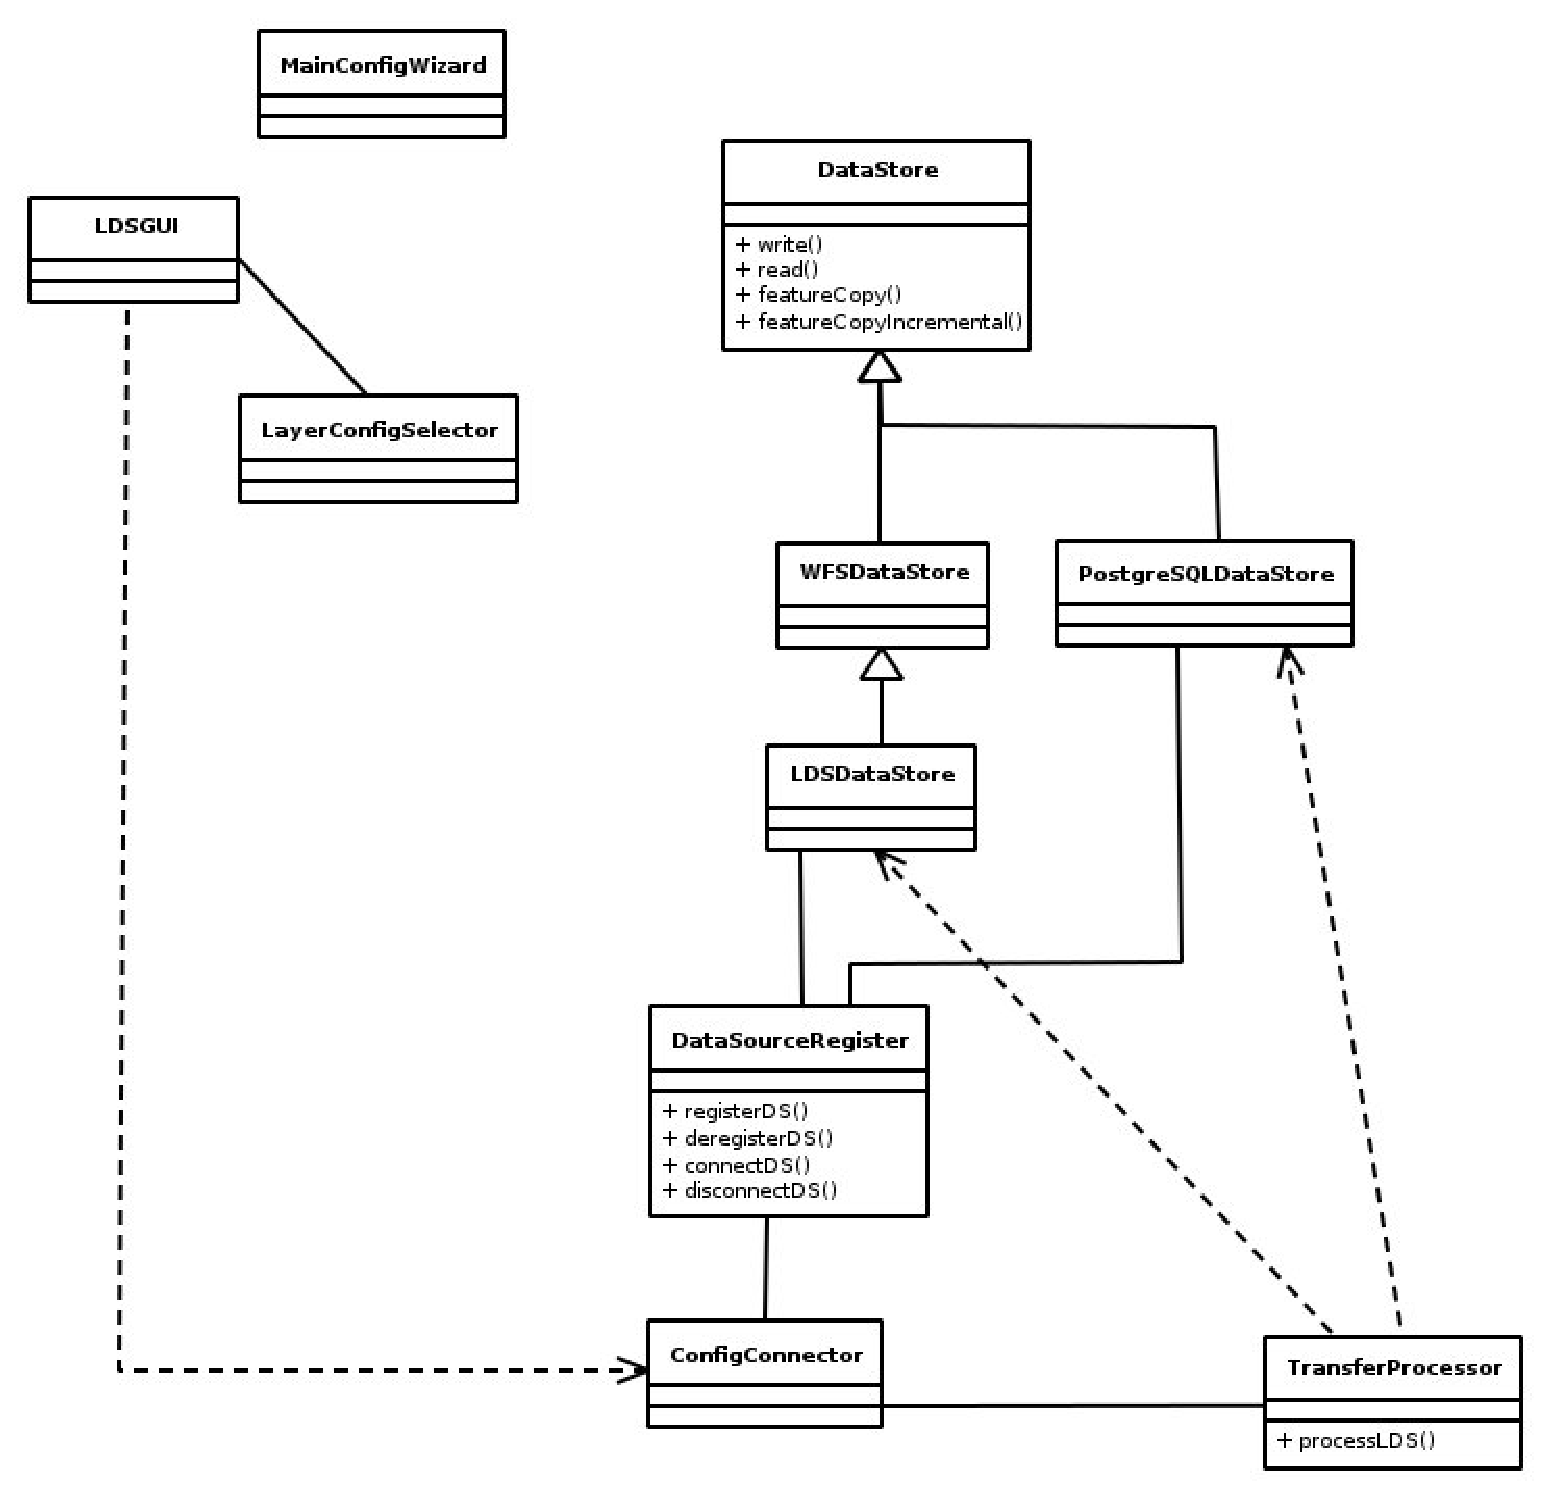
\includegraphics[width=\textwidth]{/home/jramsay/git/LDS/LDSReplicate/doc/LDSR_class.eps}
  \caption{LDSR Class Diagram}
  \label{fig:ClassDiagram}
\end{figure}

Responsibilities that cannot be handled generically are passed off to driver
related subclasses. For example, table index creation is performed directly in
SQL\footnote{GDAL does not provide an API for indexing functions, nor are these
provided in the drivers themselves} and must take into account the different
dialects for their respective databases. the index command in SQL Server is;

\begin{lstlisting}
CREATE SPATIAL INDEX <indexname> ON <tablename> WITH (BOUNDING_BOX=(XMIN=<xmin>,YMIN=<ymin>,XMAX=<xmax>,YMAX=<ymax>))
\end{lstlisting}

In PostgreSQL however that same command takes the form;

 \begin{lstlisting}
CREATE INDEX <indexname> ON <tablename> USING GIST(<spatialcolumnname>)
\end{lstlisting}

Individual DataStore objects are initialised and registered in the
DatasourceRegister ensuring these are not held open prohibiting connection from
external applications. These connection instances are in turn passed to a
\lstinline|TransferProcessor| instance to build a replication plan. Depending on
provided (stored) dates the TP checks configuration parameters, layer
availability and configures a connection string. It then calls the 
\lstinline|DataStore.write()| method which starts a \lstinline|featureCopy|
operation. Retries and paging are handled at this stage.
Feature insertion is done by cloning a `partial' feature from the original and
populating it with selected LDS field then using the clone to create a new
feature in the destination.

incremental update/delete

\section*{Maintenence Functions}

\subsection*{Module Addition}
In order to build a new DataStore module simply subclass the primary DataStore
class or one of its gerenalised subclasses, \lstinline|WFSDataStore| or
\lstinline|ESRIDataStore|. The functions determining the format of connection
strings, \lstinline|destinationURI()|, \lstinline|sourceURI()| and the function
determining the driver version number \lstinline|versionCheck()| will have to be written. 
Additionally, any functions that make use of raw SQL
to perform an actions will need to be written in their respective driver's
recognised format. \lstinline|buildIndex()| is an example of a function
rewritten sepecifically for differing driver types.
\lstinline|getLayerOptions()| and \lstinline|getConfigOptions()| may also be
added if the driver yoyu are adding has specific config requirements.

Integrating the new module into the existing codebase will require adding extra
members to any driver lists. The primary for driver references can be found in 
\begin{lstlisting}
DRIVER_NAMES =
	{'pg':'PostgreSQL',
	'ms':'MSSQLSpatial',
	'sl':'SQLite',
	'fg':'FileGDB'}
\end{lstlisting}

Substituting a new module name (making sure to use the ODR driver name) and
shortcut will take care of many interactions in the code places where this
cannot be factored out include: 
The \lstinline|MainConfigWizard| which will need a new \lstinline|QWizardPage|
where the user can enter new connection details.
The \lstinline|ReadConfig| class will have to have a new function to read these
new configuration parameters.
The \lstinline|ConfigWrapper| class will have to reference the new
\lstinline|ReadConfig| function so that saved user input can be merged
with default values.
To set up those default values a new entry will have to be added to the
template.conf file so that meaningful defaults or user prompts can be returned.


\subsection*{WFS DS Module Addition}
Addition of a module doing essentially the same job as the LDSDataStore module
but pointing at a different address falls outside the definition of an LDS
replication script but it is likely that extensions to LDS or other providers
using the LDS framework could utilise this script to duplicate data. the obvious
example here is \emph{MfE} who share the LDS platform but identify themselves
through a unique URL.

Adding a module here follows the same principles as adding a module above but
the immediate superclass of such a module is \lstinline|WFSDataStore|. In the
case of \emph{MfE}, changes will need to be made to the base URL but modifications may
need to be made in the \lstinline|RequestBuilder| class dpending on the WFS
version being employed and the layer naming scheme\footnote{While LDS uses a
`v:x\#\#\#' naming scheme a future version (WFS2.0) will employ
`linz-layer:\#\#\#' and \emph{MfE} will be using the prefix `mfe-layer:\#\#\#'}.






 \end{document}